\section{Baseline with Middleware (90 pts)\label{sec:3}}

    This experiment extends on the design of experiment \ref{subsec:2_one-server} by introducing one and two middlewares
    into the system. The middleware can be configured to have a variable amount of worker threads where each worker
    thread handles one paired request-reply operation. This parameter is also considered in the evaluation. The
    configurations are listed in table \ref{tab:30_setup}.

    \begin{table}
        \scriptsize{
            \begin{tabular}{|l|c|}
                \hline Number of servers                & 1 \\
                \hline Number of client machines        & 3 \\
                \hline Instances of memtier per machine & 1 (3.1) / 2 (3.2) \\
                \hline Threads per memtier instance     & 2 (3.1) / 1 (3.2) \\
                \hline Virtual clients per thread       & [1, 2, 4, 8, 16, 32, 48] \\
                \hline Workload                         & Write-Only and Read-Only \\
                \hline Multi-Get behavior               & N/A \\
                \hline Multi-Get size                   & N/A \\
                \hline Number of middlewares            & 1 (3.1) / 2 (3.2) \\
                \hline Worker threads per middleware    & [8, 16, 32, 64]  \\
                \hline
            \end{tabular}
        }
            \caption{Experimental parameters for experiments 3.1 and 3.2.\label{tab:30_setup}}
    \end{table}

    \subsection{One Middleware\label{subsec:3_one-middleware}}

        This experiment is similar to experiment \ref{subsec:2_one-server}, but here each \cli{} connects to the single
        instance of \mw{} which itself connects to the single instance of \srv{}.

        \begin{figure*}
            \vspace*{-.5\baselineskip}
            \makebox[1\linewidth][c]{%
                \centering
                \begin{subfigure}[t!]{0.55\textwidth}
                    \centering
                    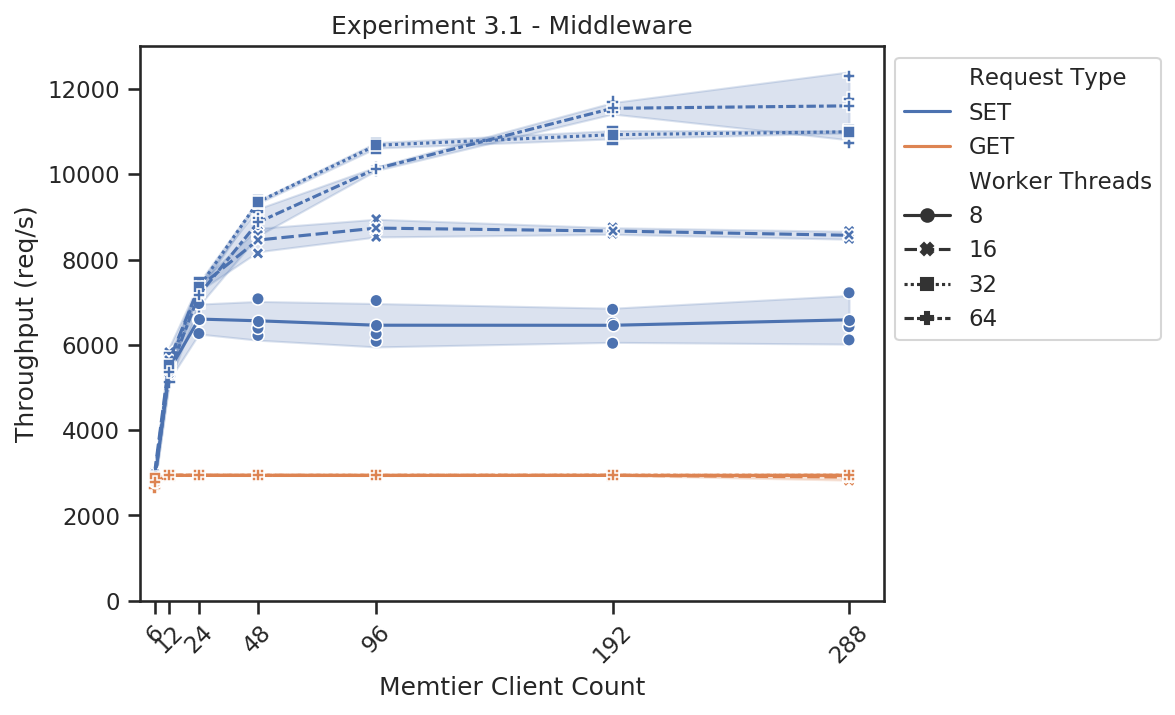
\includegraphics[width=1\textwidth]{../data_analysis/figures/3-1_mw_throughput.png}
                    \caption{Request throughput.\label{fig:single_mw_tp}}
                \end{subfigure}
                \begin{subfigure}[t!]{0.55\textwidth}
                    \centering
                    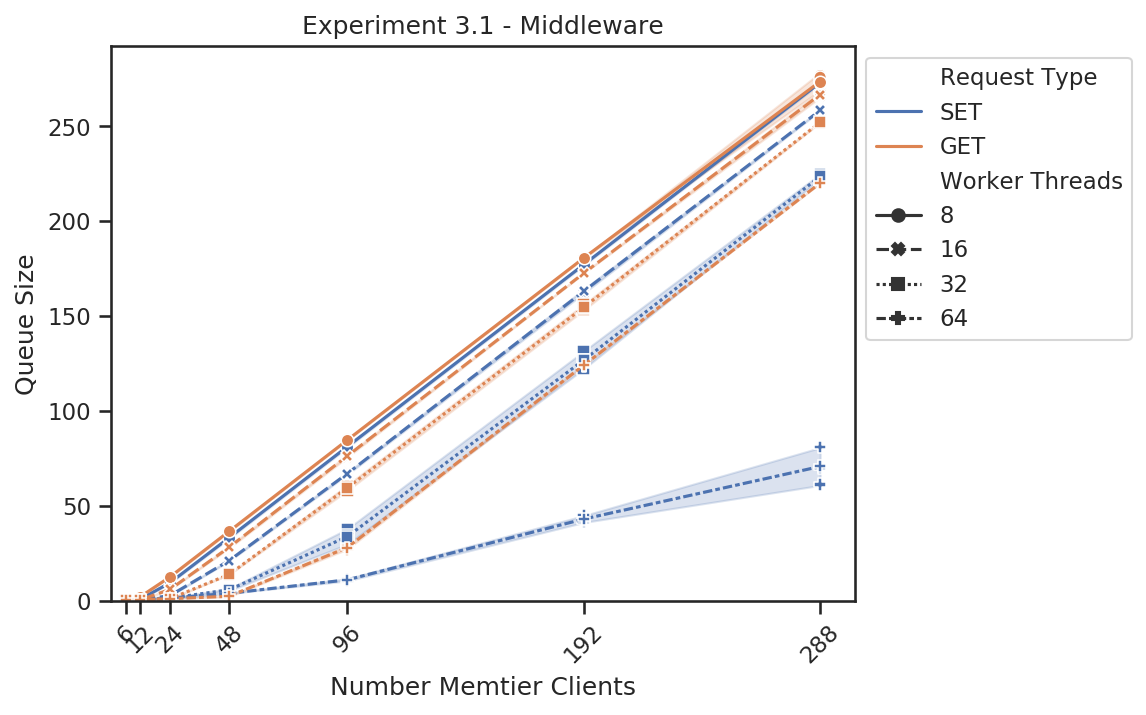
\includegraphics[width=1\textwidth]{../data_analysis/figures/3-1_mw_queue-size.png}
                    \caption{Queue sizes.\label{fig:single_mw_qs}}
                \end{subfigure}
            }
            \makebox[1\linewidth][c]{%
                \centering
                \begin{subfigure}[t!]{0.55\textwidth}
                    \centering
                    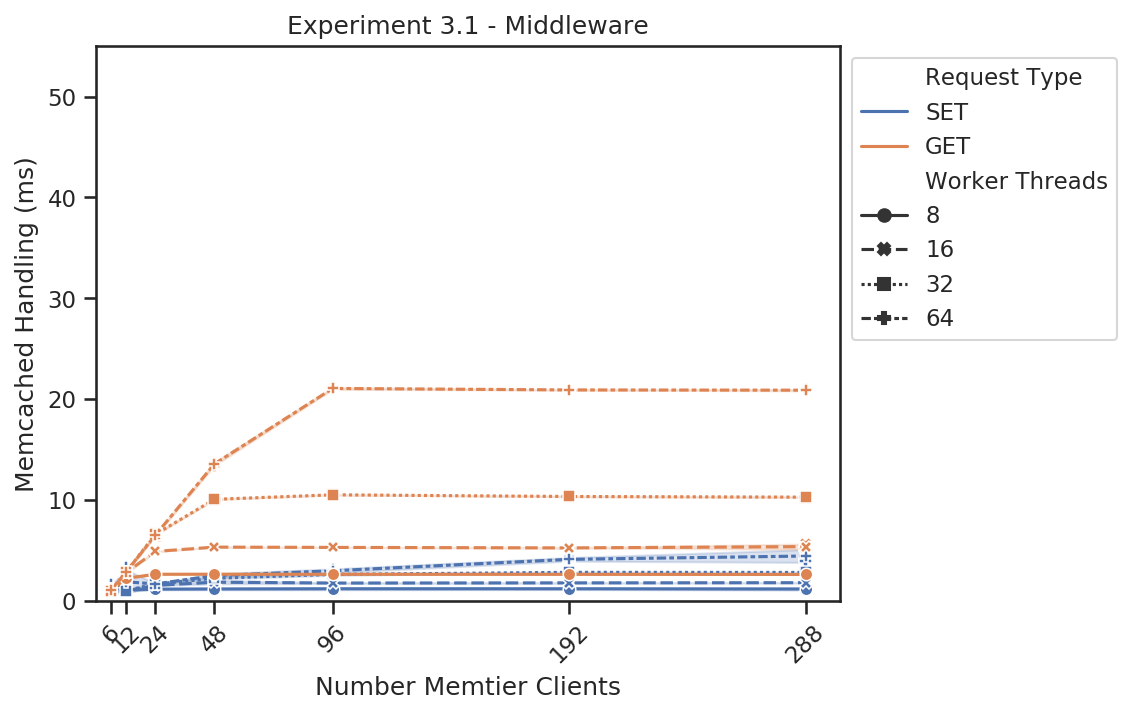
\includegraphics[width=1\textwidth]{../data_analysis/figures/3-1_mw_mc-comm-time.png}
                    \caption{Memcached communication time.\label{fig:single_mw_mct}}
                \end{subfigure}
                \begin{subfigure}[t!]{0.55\textwidth}
                    \centering
                    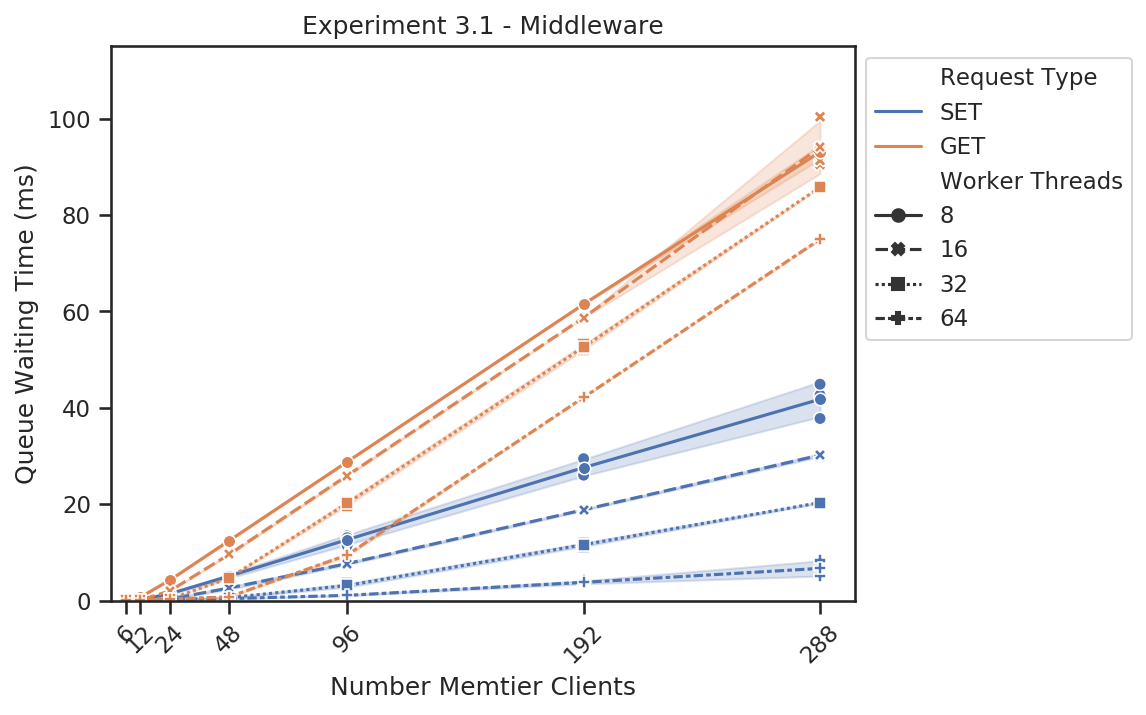
\includegraphics[width=1\textwidth]{../data_analysis/figures/3-1_mw_queue-wait-time.png}
                    \caption{Queue waiting time.\label{fig:single_mw_qwt}}
                \end{subfigure}
            }
            \makebox[1\linewidth][c]{%
                \centering
                \begin{subfigure}[t!]{0.55\textwidth}
                    \centering
                    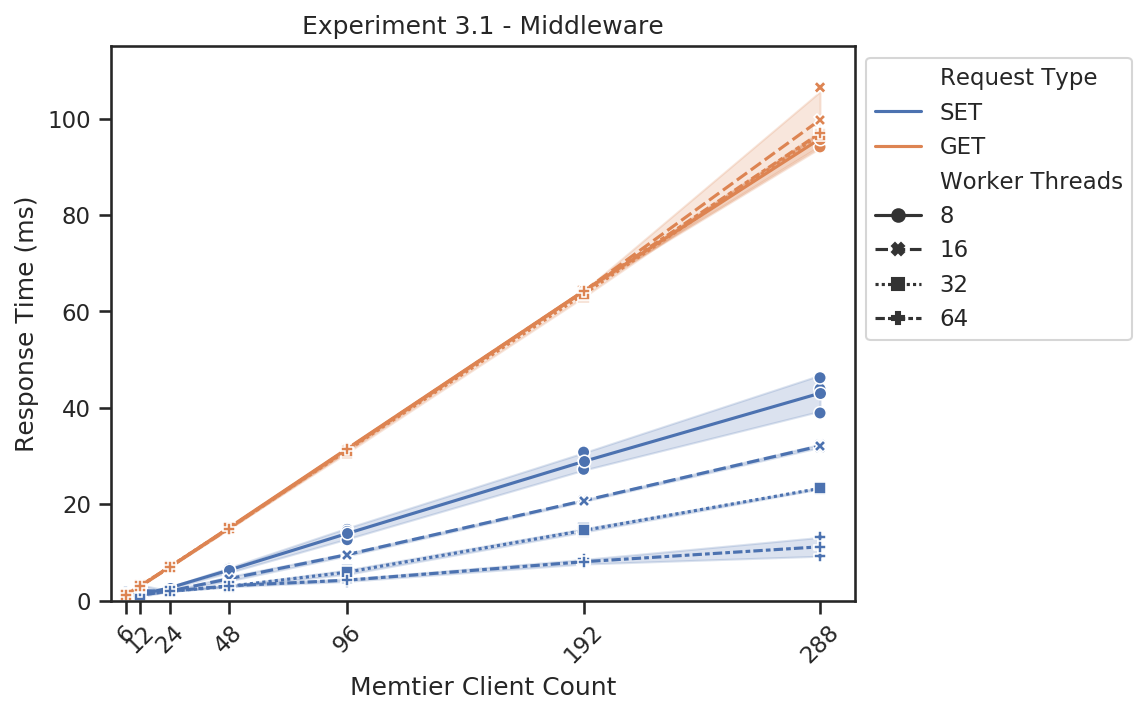
\includegraphics[width=1\textwidth]{../data_analysis/figures/3-1_mw_response_time.png}
                    \caption{Response times.\label{fig:single_mw_rt}}
                \end{subfigure}
            }
            \caption{\mw{} statistics based on SET and GET requests for various amounts of worker threads and active
                     clients.\label{fig:single_mw_all}}
        \end{figure*}

        \subsubsection{Explanation\label{subsubsec:3_one-middleware_summary}}

            Comparing the throughput of GETs with the baseline experiment only a small change in performance for 6
            clients is observed (the performance not reaching the stable phase which happens for 12 and more clients).
            The throughput oof GET requests behaves most similarly to the baseline with 64 worker threads yet the
            throughput for 32 worker threads is in general higher for 48 and 96 connected clients. This observation will
            be discussed in the following paragraphs and explained with more data. It can be inferred that the
            throughput of a single client is limited around 12000 requests, a contrast to the measured 15800 without the
            use of a middleware. This limit occurs for 192 virtual clients. The throughput being lower for fewer worker
            threads is reasonable and the non-linear scaling highly likely due to the fact that \mw{}s have only 8
            physical cores.

            The response rates are also similar to the baseline experiment in general with SETs having a smaller
            response time than GETs. Looking at the constituents of response time (with detailed timings for queue
            waiting times and memcached communication and respective packet handling time) it can be observed that for
            few worker threads and many clients queue times grow from a certain point quasi-linear. The memcached
            communication and packet handling time does flatten though. The height of flattened sections can be
            explained due to thread scheduling (the flattened lines are all separated by an even delta proportional to
            the number of worker threads divided by the core count of the machine). The reasoning for flattening due to
            the fact that there is sufficient load on the middleware to 

            As such the total response time of the middleware is for a large amount of clients and few worker threads
            determined by the queueing time and for few clients and many worker threads determined mostly by the
            communication time with memcached.

            Coming back to the open question of why 32 worker threads perform better than 64 for 48 and 96 clients
            requires the use of the queue where requests are stored. As long as this queue is not always at least the
            size of worker threads some threads don't have anything to do. This results in an effectively smaller
            throughput as only some threads are working but the threads waiting for a new element contend on a shared
            lock on the queue. Only once the queue at 192 clients approaches 64 elements does the middleware become more
            saturated and is even more so at 288 clients. It is very close to the point of complete saturation when
            looking at the queue size, yet no real increase in throughput was measured. As the standard deviation for
            288 clients and 64 worker threads is rather large compared to previous results for it the assumption can be
            made that beyond a certain amount of threads and connections the cloud environment is not scaling well.

            Overall it can be concluded that for 8\textendash 32 clients the maximal saturation point has been reached
            and for 64 threads the saturation point is within a few percent or has been reached.

    \subsection{Two Middlewares\label{subsec:3_two-middlewares}}

        This experiment is virtually identical to the previous experiment with the change of each \srv{} running two
        single-threaded memtier instances where the second connects to the newly added second \mw{}.

        \begin{figure*}
            \vspace*{-.5\baselineskip}
            \makebox[1\linewidth][c]{%
                \centering
                \begin{subfigure}[t!]{0.55\textwidth}
                    \centering
                    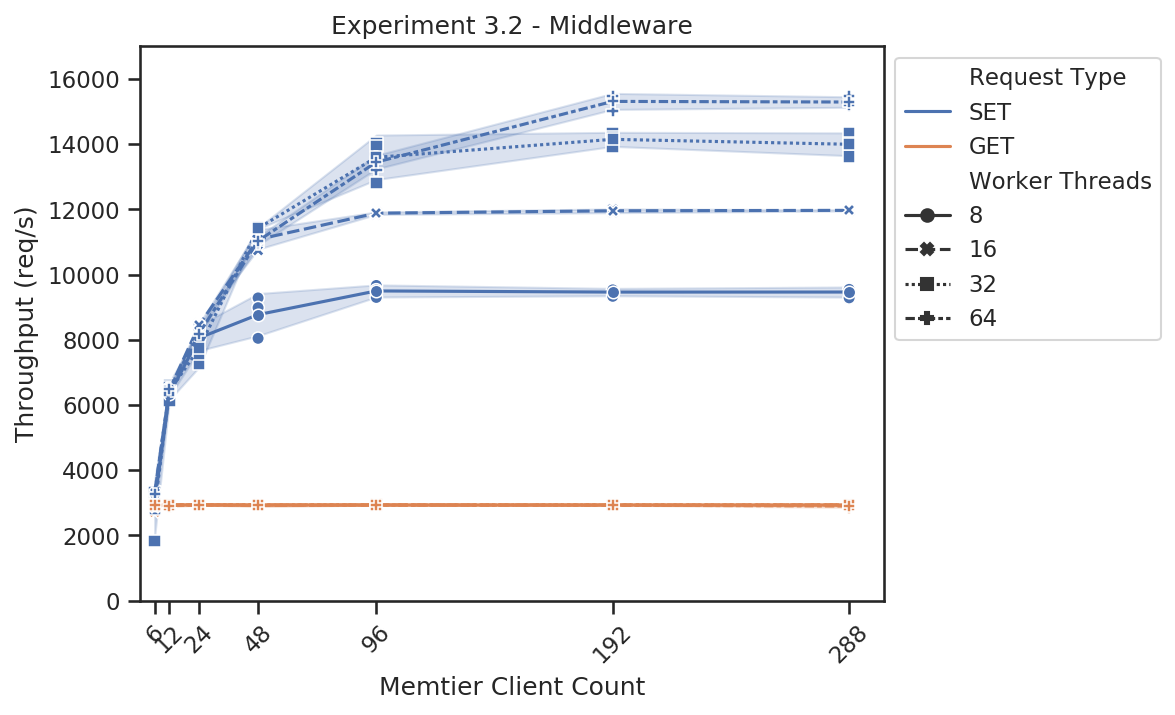
\includegraphics[width=1\textwidth]{../data_analysis/figures/3-2_mw_throughput.png}
                    \caption{Request throughput.\label{fig:double_mw_tp}}
                \end{subfigure}
                \begin{subfigure}[t!]{0.55\textwidth}
                    \centering
                    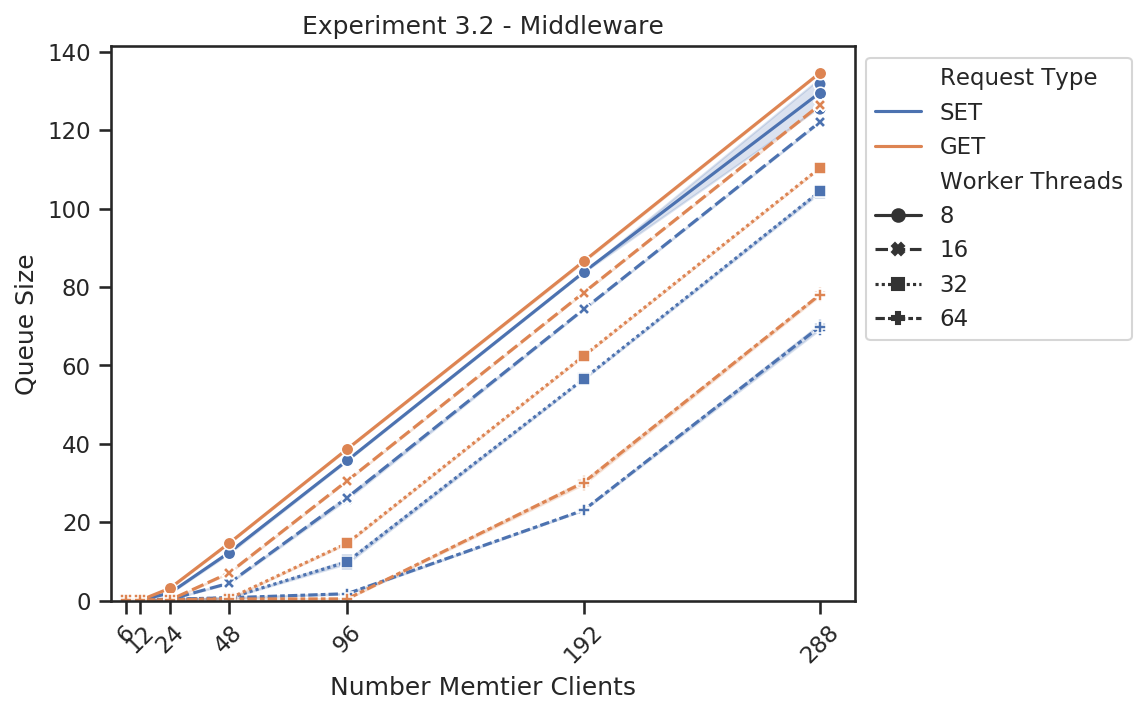
\includegraphics[width=1\textwidth]{../data_analysis/figures/3-2_mw_queue-size.png}
                    \caption{Queue sizes.\label{fig:double_mw_qs}}
                \end{subfigure}
            }
            \makebox[1\linewidth][c]{%
                \centering
                \begin{subfigure}[t!]{0.55\textwidth}
                    \centering
                    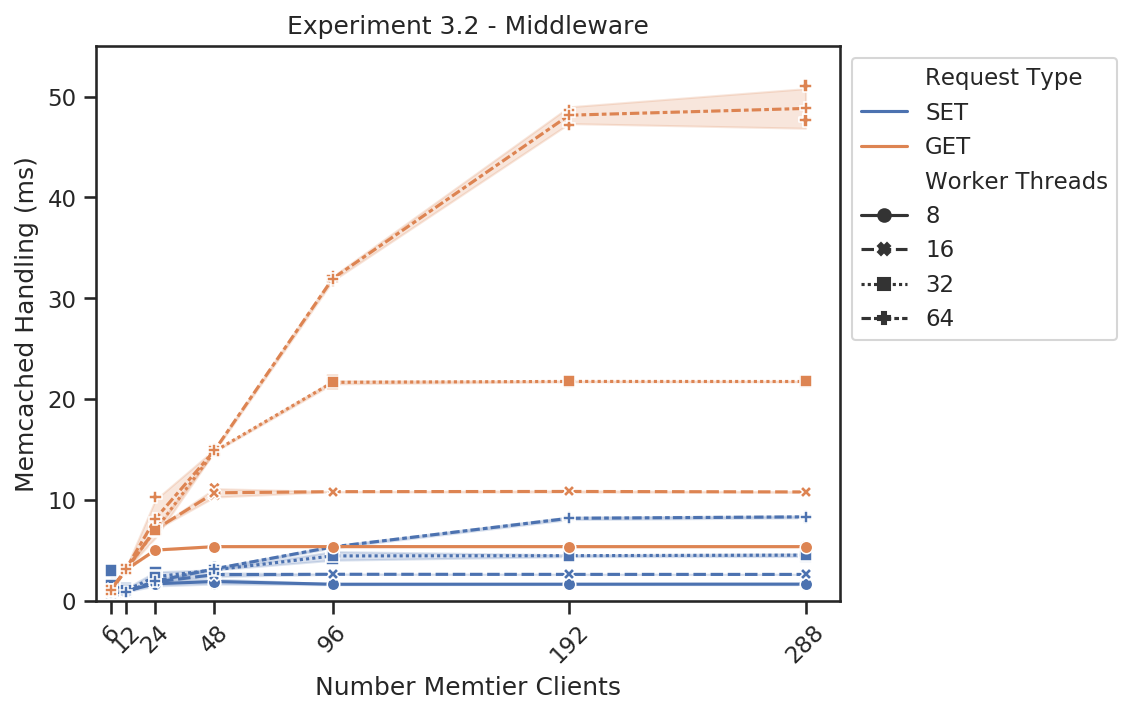
\includegraphics[width=1\textwidth]{../data_analysis/figures/3-2_mw_mc-comm-time.png}
                    \caption{Memcached communication time.\label{fig:double_mw_mct}}
                \end{subfigure}
                \begin{subfigure}[t!]{0.55\textwidth}
                    \centering
                    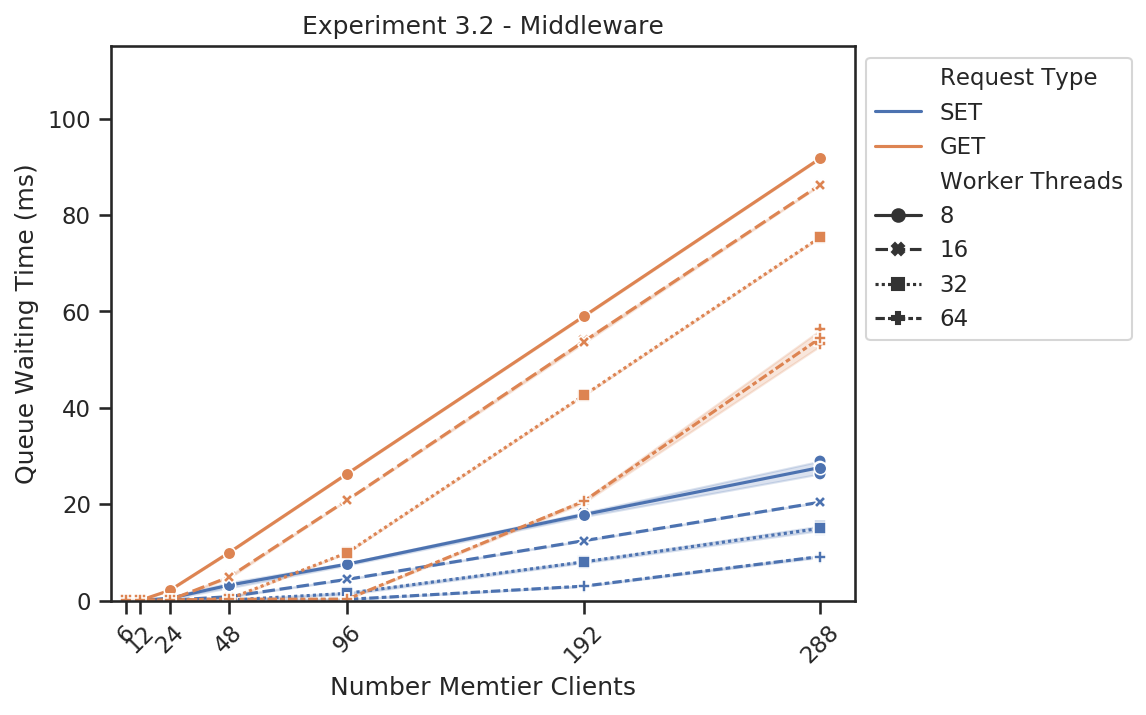
\includegraphics[width=1\textwidth]{../data_analysis/figures/3-2_mw_queue-wait-time.png}
                    \caption{Queue waiting time.\label{fig:double_mw_qwt}}
                \end{subfigure}
            }
            \makebox[1\linewidth][c]{%
                \centering
                \begin{subfigure}[t!]{0.55\textwidth}
                    \centering
                    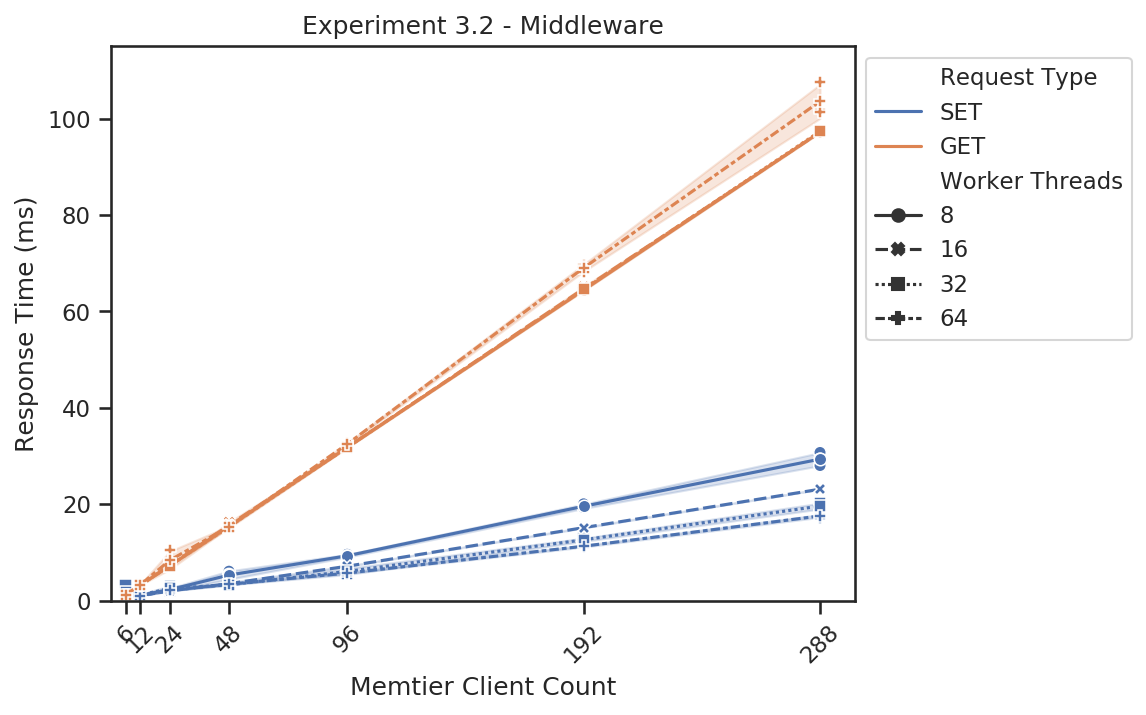
\includegraphics[width=1\textwidth]{../data_analysis/figures/3-2_mw_response_time.png}
                    \caption{Response times.\label{fig:double_mw_rt}}
                \end{subfigure}
            }
            \caption{\mw{} statistics based on SET and GET requests for various amounts of worker threads and active
                     clients.\label{fig:double_mw_all}}
        \end{figure*}

        \subsubsection{Explanation\label{subsubsec:3_two-middlewares_summary}}

            % Comparing the throughput of GETs with the baseline experiment only a small change in performance for 6
            % clients is observed (the performance not reaching the stable phase which happens for 12 and more clients).
            % The throughput oof GET requests behaves most similarly to the baseline with 64 worker threads yet the
            % throughput for 32 worker threads is in general higher for 48 and 96 connected clients. This observation will
            % be discussed in the following paragraphs and explained with more data. It can be inferred that the
            % throughput of a single client is limited around 12000 requests, a contrast to the measured 15800 without the
            % use of a middleware. This limit occurs for 192 virtual clients. The throughput being lower for fewer worker
            % threads is reasonable and the non-linear scaling highly likely due to the fact that \mw{}s have only 8
            % physical cores.
            %
            % The response rates are also similar to the baseline experiment in general with SETs having a smaller
            % response time than GETs. Looking at the constituents of response time (with detailed timings for queue
            % waiting times and memcached communication and respective packet handling time) it can be observed that for
            % few worker threads and many clients queue times grow from a certain point quasi-linear. The memcached
            % communication and packet handling time does flatten though. The height of flattened sections can be
            % explained due to thread scheduling (the flattened lines are all separated by an even delta proportional to
            % the number of worker threads divided by the core count of the machine). The reasoning for flattening due to
            % the fact that there is sufficient load on the middleware to 
            %
            % As such the total response time of the middleware is for a large amount of clients and few worker threads
            % determined by the queueing time and for few clients and many worker threads determined mostly by the
            % communication time with memcached.
            %
            % Coming back to the open question of why 32 worker threads perform better than 64 for 48 and 96 clients
            % requires the use of the queue where requests are stored. As long as this queue is not always at least the
            % size of worker threads some threads don't have anything to do. This results in an effectively smaller
            % throughput as only some threads are working but the threads waiting for a new element contend on a shared
            % lock on the queue. Only once the queue at 192 clients approaches 64 elements does the middleware become more
            % saturated and is even more so at 288 clients. It is very close to the point of complete saturation when
            % looking at the queue size, yet no real increase in throughput was measured. As the standard deviation for
            % 288 clients and 64 worker threads is rather large compared to previous results for it the assumption can be
            % made that beyond a certain amount of threads and connections the cloud environment is not scaling well.
            %
            % Overall it can be concluded that for 8\textendash 32 clients the maximal saturation point has been reached
            % and for 64 threads the saturation point is within a few percent or has been reached.

    \subsection{Summary\label{subsec;3_summary}}

    \begin{table}
          \def\sym#1{\ifmmode^{#1}\else\(^{#1}\)\fi}%
        \footnotesize{
            % \centering
            % \begin{subfigure}[t!]{0.45\textwidth}
                \centering
                \begin{tabular}{l*{10}{c}}
                    \toprule
                    & & \multicolumn{2}{c}{Throughput}  & \multicolumn{2}{c}{Response Time} &
                    \multicolumn{2}{c}{Queueing Time} & \multicolumn{2}{c}{Miss Rate} \\
                    \cmidrule(lr){3-4}\cmidrule(lr){5-6}
                    \cmidrule(lr){7-8}\cmidrule(lr){9-10}
                    Type & Machine & Exp 3.1  & Exp 3.2  & Exp 3.1 & Exp 3.2 & Exp 3.1 & Exp 3.2 & Exp 3.1 & Exp 3.2 \\
                    \midrule
                    GET  & \cli    & 2936.58  & 2923.27  & 4.08    & 2.06    & N/A     & N/A     & 0.00    & 0.00 \\
                         & \mw     & 2939.02  & 2928.91  & 3.04    & 1.24    & 0.72    & 0.05    & 0.00    & 0.00 \\
                    \addlinespace
                    SET  & \cli    & 11548.63 & 15305.89 & 16.73   & 12.55   & N/A     & N/A     & 0.00    & 0.00 \\
                         & \mw     & 11545.56 & 15309.86 & 8.07    & 11.38   & 3.80    & 3.03    & 0.00    & 0.00 \\
                    \bottomrule
                \end{tabular}
                \caption{Evaluation of maximum throughputs for one and two \mw{}s in the system.\label{tab:3_throughput-summary}}
            % \end{subfigure}
        }
    \end{table}

        % \begin{table}
        %     \begin{tabular}{|l|p{2cm}|p{2cm}|p{2cm}|p{2cm}|} % Read 12 clients, writes at 192
        %         \hline                                & Throughput        & Response time & Average time in queue & Miss rate \\
        %         \hline Reads: Measured on middleware  & 2939.02 [3.57]    & 3.04 [0.01]   & 0.72                  & 0.00 [0.00] \\
        %         \hline Reads: Measured on clients     & 2936.58 [3.59]    & 4.08 [0.00]   & n/a                   & 0.00 [0.00] \\
        %         \hline Writes: Measured on middleware & 11545.56 [134.28] & 8.07 [0.47]   & 3.80 [0.31]           & n/a \\
        %         \hline Writes: Measured on clients    & 11548.63 [136.48] & 16.73 [0.32]  & n/a                   & n/a \\
        %         \hline
        %     \end{tabular}
        %     \caption{Evaluation of maximum throughputs of 3:1:1 (Client:Middleware:Server). In square brackets the standard
        %              deviation is given, numbers are rounded to two decimal places.\label{tab:31_throughput}}
        % \end{table}
        %
        % \begin{table}
        %     \begin{tabular}{|l|p{2cm}|p{2cm}|p{2cm}|p{2cm}|} % read 6 clients, writes at 192
        %         \hline                                & Throughput        & Response time & Average time in queue & Miss rate \\
        %         \hline Reads: Measured on middleware  & 2928.91 [13.34]   & 1.24 [0.01]   & 0.05 [0.00]           & 0.00 [0.00] \\
        %         \hline Reads: Measured on clients     & 2923.27 [13.33]   & 2.05 [0.01]   & n/a                   & 0.00 [0.00] \\
        %         \hline Writes: Measured on middleware & 15309.86 [245.75] & 11.38 [0.19]  & 3.03 [0.05]           & n/a       \\
        %         \hline Writes: Measured on clients    & 15305.89 [245.82] & 12.55 [0.20]  & n/a                   & n/a       \\
        %         \hline
        %     \end{tabular}
        %     \caption{Evaluation of maximum throughputs of 3:2:1 (Client:Middleware:Server). In square brackets the standard
        %              deviation is given, numbers are rounded to two decimal places.\label{tab:32_throughput}}
        % \end{table}

        As already mentioned in the baseline experiments without the use of a middleware the evaluation of GET and SET
        requests follows similar base criteria, namely throughput and response time. In case where these are not
        sufficient, it is possible to use the middleware's instrumentation and deduce the system behaviour from them.

        In the case of GET requests the behaviour between experiments \ref{subsec:2_one-server},
        \ref{subsec:3_one-middleware} and \ref{subsec:3_two-middlewares} is comparable, not the benchmarking results
        though. Oddly for six clients the system is not immediately saturated for any worker thread configuration with a
        single middleware. Only at twelve clients this saturation occurs. It is quite likely that the overhead of the
        middleware is just high enough to introduce minimal latencies in such a configuration as the system has empty
        queues and as such it is not a problem of queueing. As experiment \ref{sec:2} and \ref{sec:3} were run on two
        different instances of machines changes in benchmarking performances are expected, yet the general behaviour
        should stay comparable. This is the case for GETs in our experiments as well as for SETs.

        In the case for SET requests the trends with more active clients introducing more throughput does not always
        match. At some points a flattening occurs and no more throughput increases are observed. This is the point
        where the middleware slows down the system as it cannot handle more requests. There is a trend of more worker
        threads introducing more throughput. Also adding another middleware helps and actually shows to scale better
        than adding more worker threads when comparing the throughput graphs for the total amount of comparable worker
        threads between both experiments (for experiment \ref{subsec:3_two-middlewares} half the worker thread count
        must be evaluated as two middlewares are used). This is to be expected as at some point scheduling overhead on a
        single system results in slowdowns.

        For a thorough and clear evaluation of system behaviour including the internal queue sizes (and respective
        waiting times) and the memcached communication overhead need to be included.\newline
        As already observed for a given amount of worker threads the memcached communication begins to flatten for a
        certain amount of active clients. The trend is that more worker threads can handle more clients but the time to
        process grows. This aligns well with the fact that there is contention for the actual cores of the machine by
        each worker thread. As each \mw{} has 8 cores it is expected that the communication time grows linearly in the
        amount worker threads at the point of full saturation. This is also observed. The queue sizes also reflect in
        the queue waiting times appropriately for both experiments in this section. Additionally the queue sizes offer a
        good metric in evaluating the saturation of the system and aid in defining the maximum throughput for each
        configuration of worker threads. Once the queue sizes reaches the amount of worker threads there is no more more
        waiting on the next task for each worker thread but adding more elements than there are worker threads slows
        down the system as at that point no bijection exists between worker threads and items to process.

        The summary tables for throughput have been filled out with the following configurations.
        Single \mw{}: GET uses 8 worker threads and has 12 clients, SET uses 64 worker threads and has 192 clients.
        Two \mw{}s: GET uses 8 worker threads and has 6 clients, SET uses 64 worker threads and has 192 clients.

        Comparing the numbers of the summary table \ref{tab:3_throughput-summary} the behaviour of GET requests gives
        the same throughput but different response times. This is due to the fact that for the case of a single \mw{}
        twelve total clients were chosen as the maximum throughput configuration and six for the case of two \mw{}s. As
        such the response times reflect over a single request sent by each client. For double the amount of clients a
        doubling of response times is expected. The numbers match therefore when looking at an individual client from
        both configurations. The difference in the queue size is also expected as the per-worker-thread load is higher
        for experiment \ref{subsec:3_one-middleware}.\newline
        For SET requests an increase in performance is observed using two \mw{}s with a corresponding decrease of the
        response time measured at memtier. The difference between response times observed at the middleware and memtier
        are much larger for the case of a single middleware. A reasonable explanation could be related to the middleware
        receiving SET requests with a single thread. If multiple requests buffer on the socket then multiple complete
        requests can be processed much quicker from it than having to receive each TCP alone. Both systems do have the
        same queue waiting time so the worker threads are performing similarly well. This strengthens the assumption
        that OS-side buffering of TCP packets occur and not somewhere measurable within the middleware.

        As the middleware doesn't include the full response time the interactive law doesn't hold for this aspect. For
        the throughput measured it describes much better the response time measured at memtier and as such it can be
        used to derive the actual response time of the system. Two examples, one using the throughput to measure the
        response time and the other to measure the throughput can be seen in figure \ref{fig:il_violation-example}.

        \begin{figure*}
            \vspace*{-.5\baselineskip}
            \makebox[1\linewidth][c]{%
                \centering
                \begin{subfigure}[t!]{0.55\textwidth}
                    \centering
                    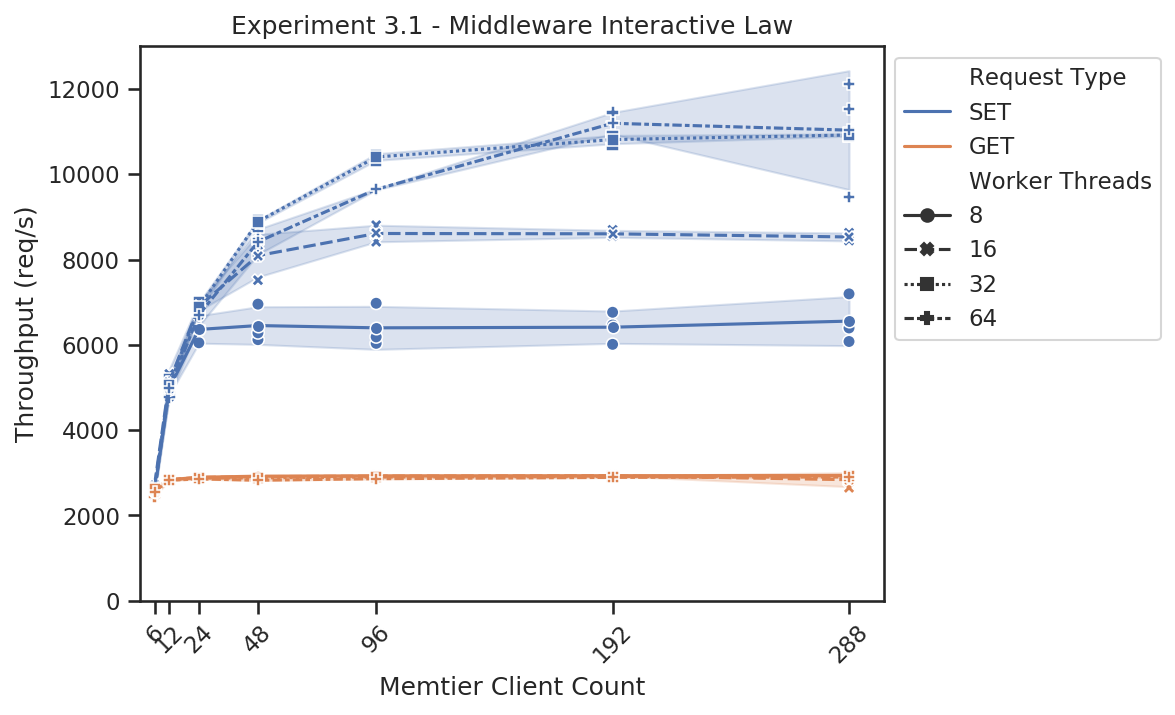
\includegraphics[width=1\textwidth]{../data_analysis/figures/3-1_mw_throughput-il.png}
                    \caption{\mw{} interactive law deriving the request throughput.\label{fig:mw_tp-il}}
                \end{subfigure}
                \begin{subfigure}[t!]{0.55\textwidth}
                    \centering
                    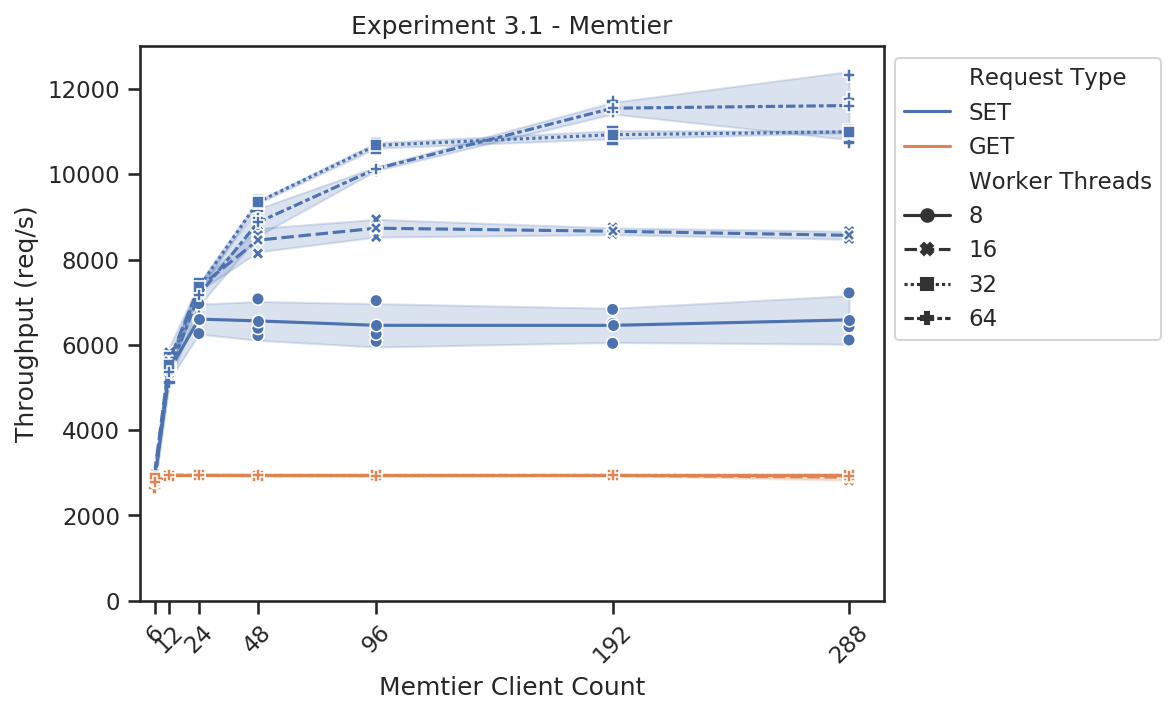
\includegraphics[width=1\textwidth]{../data_analysis/figures/3-1_mt_throughput.png}
                    \caption{\cli{} measured request throughput.\label{fig:mt_tp}}
                \end{subfigure}
            }
            \makebox[1\linewidth][c]{%
                \centering
                \begin{subfigure}[t!]{0.55\textwidth}
                    \centering
                    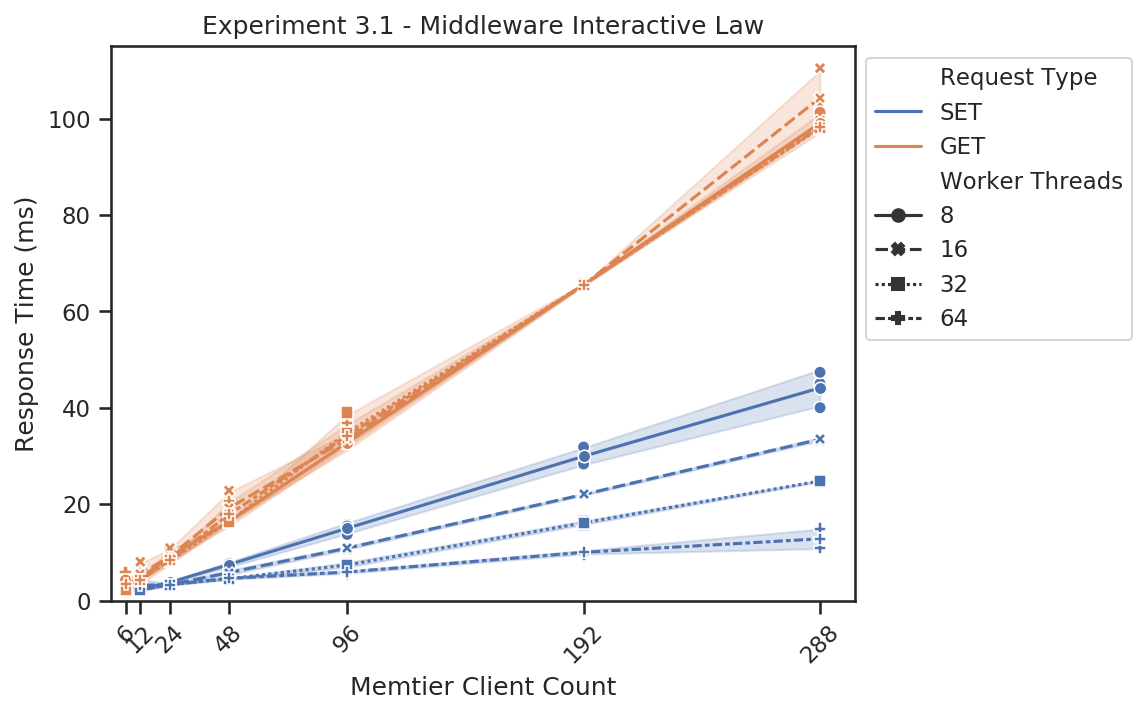
\includegraphics[width=1\textwidth]{../data_analysis/figures/3-1_mw_response-time-il.png}
                    \caption{\mw{} interactive law deriving the response time.\label{fig:mw_rt-il}}
                \end{subfigure}
                \begin{subfigure}[t!]{0.55\textwidth}
                    \centering
                    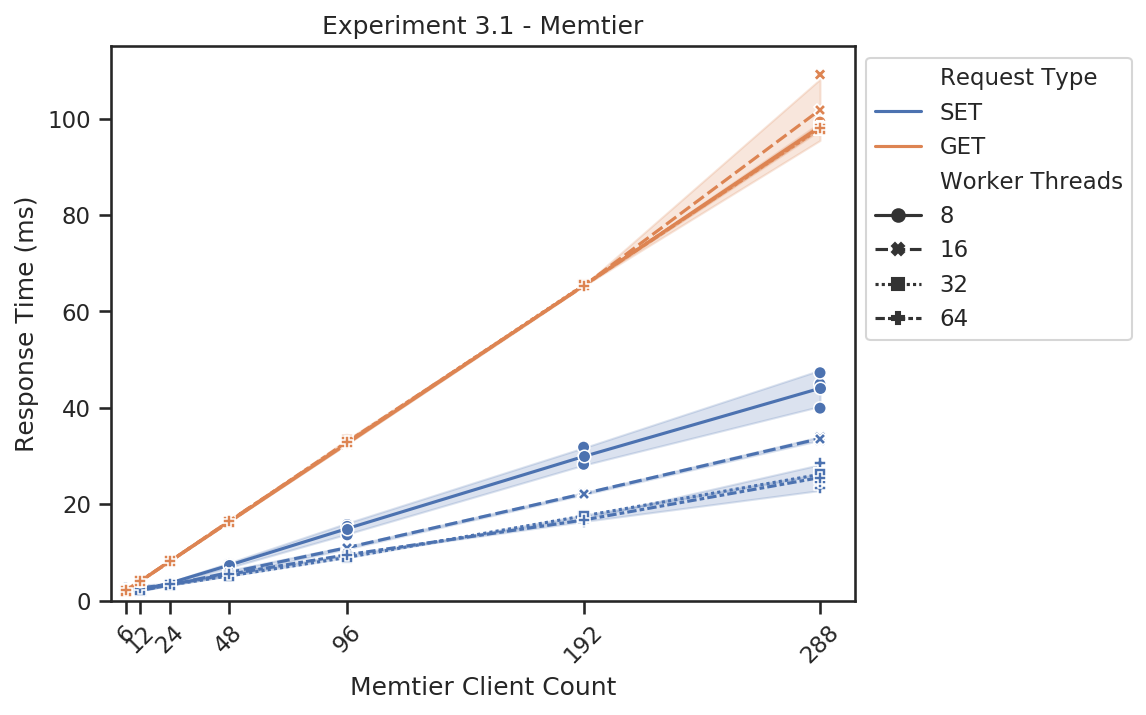
\includegraphics[width=1\textwidth]{../data_analysis/figures/3-1_mt_response_time.png}
                    \caption{\cli{} measured response times.\label{fig:mt_rt}}
                \end{subfigure}
            }
            \caption{Example visualization of the violation of the interactive law when using the response time as
                     reported on the middleware and the correctness of using the throughput measured to infer full
                     system response times.\label{fig:il_violation-example}}
        \end{figure*}
